	\section{Гомологичная рекомбинация. Модель Холлидея.
		Гены рекомбинации (recA, ssb, ruvABC). RecA и SOS-ответ.
		Сайт-специфическая рекомбинация. 
		Рекомбинация в эукариотах. Кроссинговер.}
	
\textbf{Рекомбинация} -- возникновение новых последовательностей ДНК за счёт разрывов и пересоединений уже имеющихся молекул.
\textbf{Синаптический комплекс} -- комплекс из двух ДНК с перекрещивающимися цепями
\subsection{Гомологичная (общая) рекомбинация, модель Холидея}
Обмен участками между гомологичными (практически одинаковыми по последовательностям)  молекулам ДНК. За счёт гомологичной рекомбинации не создаются новые последовательности, а перемешиваются имеющиеяс похожие варианты одной и той же последовательности.

Характеризуется следующими стадиями (Рис \ref{pic:8_holi})
\begin{enumerate}
\item Делаются два разреза в одинаковых положениях цепи
\item Одна цепь высвобождается, за счёт RecA ищет гомологичный кусок 
\item Образуется D-loop, засчёт того, что смещённая цепь вытеснила кусок другой
\item D-loop рвётся и образуется структура Холидея
\end{enumerate}
  
 Крест Холидея может двигаться при этом в обе стороны рекомбинирующих молекул, при этом сами молекулы вращаются вокруг своей оси, а гетеродуплексный (из разных кусков) участок удлиняется или укорачивается. 
 
 При этом цепи ДНК в гетеродуплексе не обязательно комплементарны и в результате рекомбинации могут образовывать разный результат. Если неспаренные основания не репарируются, то каждая цепь даст такой же дуплекс, как у родительской ДНК, если репарация происходит, то часть одной цепи станет совпадать со второй цепью.
 
 Куски при этом можно по разному резать (см \ref{pic:8_holi} д, е )
 
 Таких структур может быть несколько, получаются из-за чего более сложные объекты
 \begin{figure}[H]
 	\centering{
 	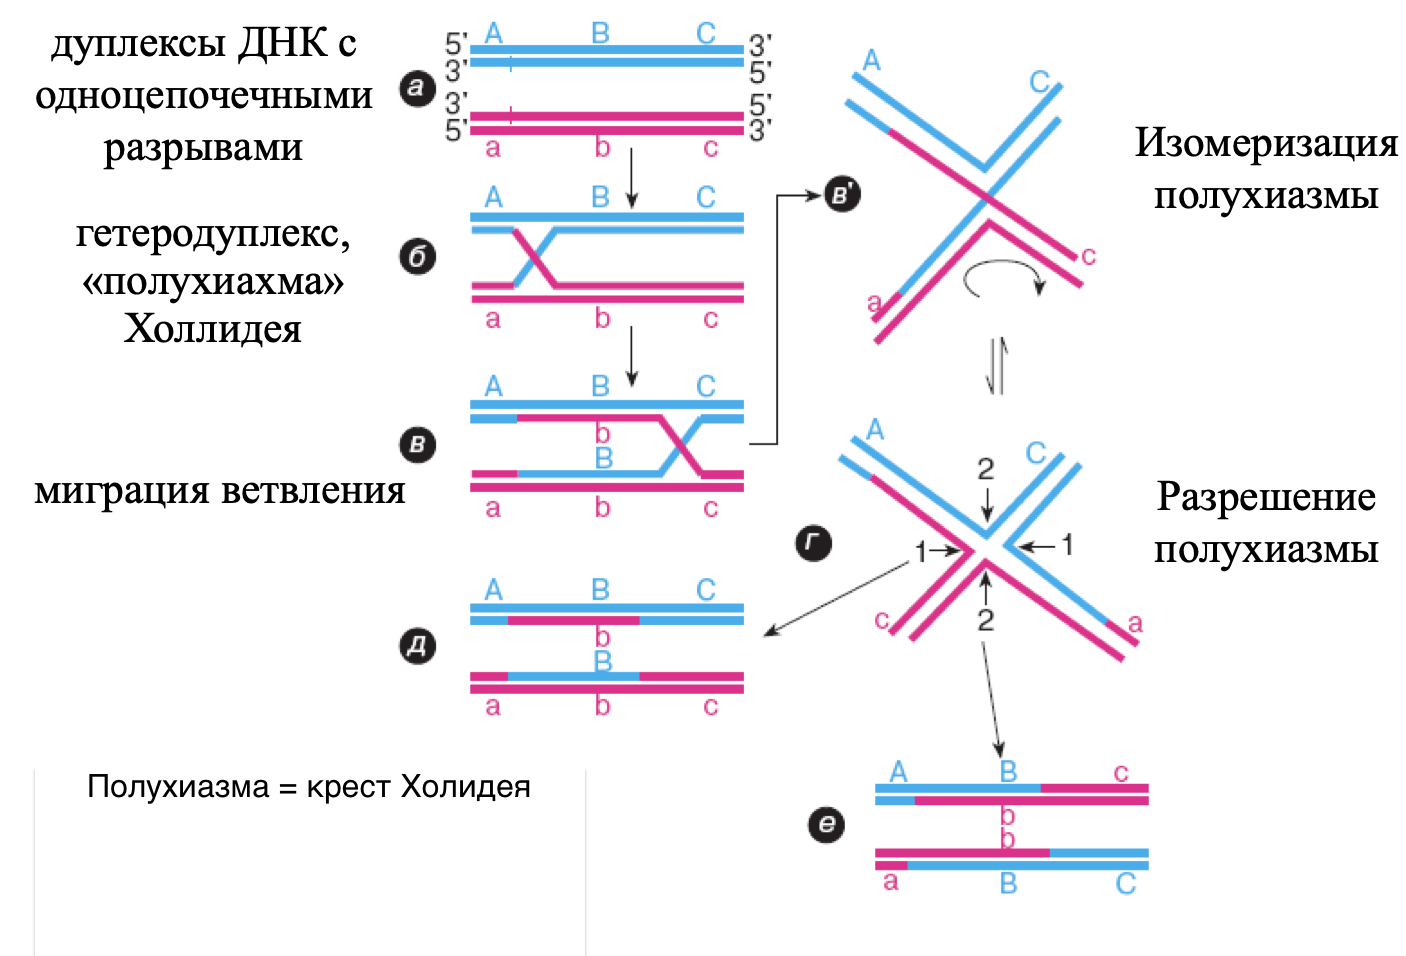
\includegraphics[scale=0.5]{8_holi.png}
 	\caption{Основные стадии общей рекомбинации}
 	\label{pic:8_holi}}
 \end{figure}
 	
\subsection{Гены рекомбинации}
\paragraph{RecA}  -- консервативный белок, который есть и у прокариотов, и у эукариотов, хотя при этом по нему можно получить мутацию. Важен для эволюции, поэтому как доп функция у бактерий -- запускает SOS-ответ. 

Умеет связываться с одноцепочечной ДНК (нарастает в сторону 3' конца) и искать гомологию, а потом переносить одноцепочечный фрагмент на двухцепочечный, который после расплетает, после чего формируется гетеродуплекс. Умеет связываться с двуцепочечной ДНК, но реже. 
\paragraph{SSB} -- Связываются с одноцепочечной ДНК и не дают ей связаться в двойную цепь, что препятствовало бы рекомбинации.Также ускоряет среднюю скорость синтеза ДНК бактериальными и архейными полимеразами..
\paragraph{ruvABC} $\ $\newline



 ruvA -- связывается со всей структурой Холидея и стабилизирует её
 
 ruvB -- белок, который вращает ДНК для продвижения креста. Тесно связывается с ruvA, поэтому вращение ДНК происходит ещё и относительно ruvA. 
 
 ruvC -- белок, который разрезает структуру Холидея симметрично с обеих сторон. У ruvC есть некоторая предпочтительная последовательность, поэтому разрезание происходит только на специфическом сайте. 
 	\begin{figure}[H]
 	\centering
 	\subfigure[a][ruvAB]{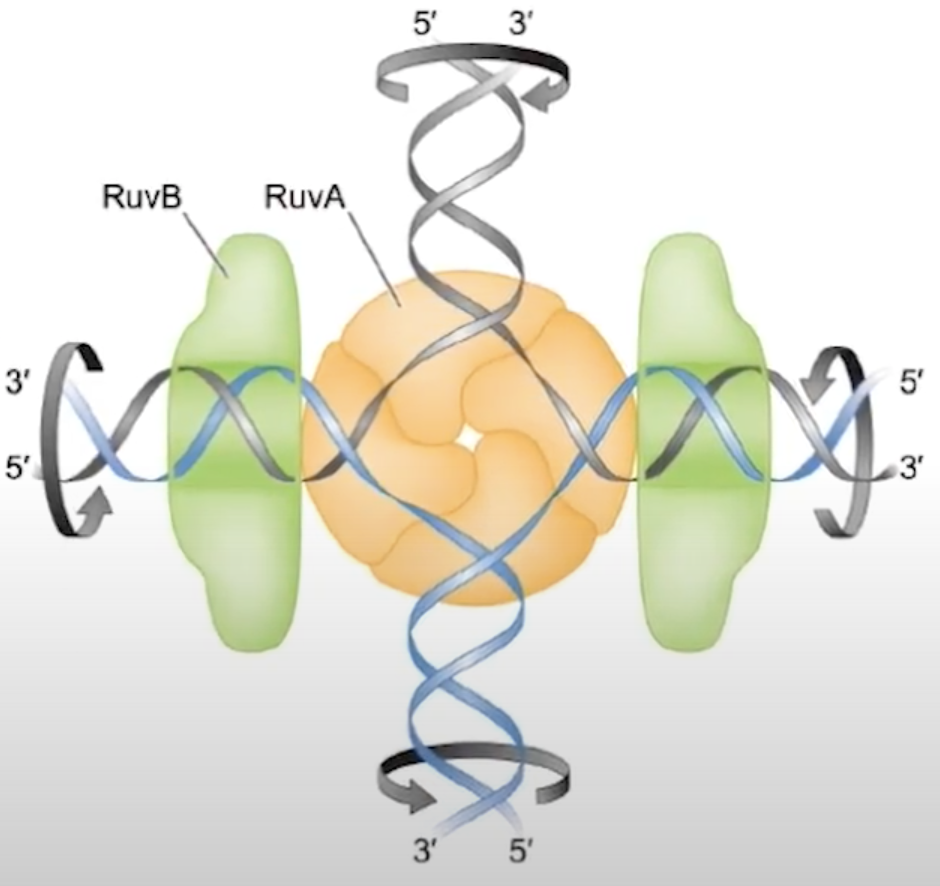
\includegraphics[scale=0.5]{8_ruvAB.png}}
 	\qquad
 	\subfigure[b][ruvC]{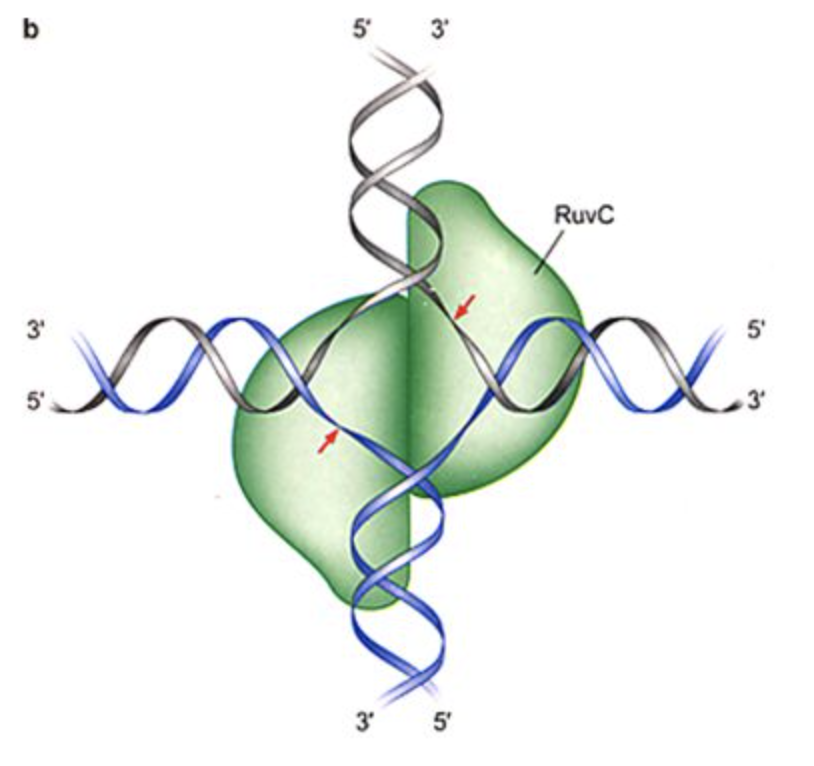
\includegraphics[scale=0.5]{8_ruvC.png}}
 \end{figure}
 	
\subsection{SOS-ответ и recA}

При малом количестве повреждений увеличивается количество uvrАBCD. 

При большом блокируется деление клеток и тем самым индуцируется синтез RecA, который нужен для рекомбинационной репарации. В активной конформации RecA стимулирует деградацию LexA (репрессора, в том числе себя и RecA, umuCD (ДНК полимераза-5), uvrABCD), после чего транскрибируются ген uvrB, продукты которого транскрибируются в эксцезионной репарации. 

Также RecA может umuCD откусывается RecA, оставляя umuC'D'

При ещё большем числе повреждений активируются umuCD, продукты которых позволяют полимеразе копировать нарушенный участок матрицы (вероятно позволяют им удлинять затравку), из-за чего больше мутаций. 
\subsection{Сайт-специфическая рекомбинация}
Не требует протяжённых участков гомологии, но требуются строго определённые последовательности ДНК и специальный ферментативный аппарат.

Происходит обычно при встраивании бактериофага в геном бактерии. 

\paragraph{Общая схема} Последовательность, которая,  способна к рекомбинации окружена специальными сайтами, которые узнаются рекомбиназой, а потом, например, меняют положение последовательности в последовательности. В зависимости от расположения сайтов рекомбинации получаются разные результаты, так как каждые сайты рекомбинации асимметричны.

Сам сайт при этом выглядит как асимметричный кусок посередине и два куска, которые одинаково читаются при прочтении с разных сторон (палиндромы). Каждые куски-палиндромы связываются с рекомбиназой, после чего вносятся разрывы в ДНК. (см Рис. \ref{pic:8_ssrec}). Сначала отрывается одна цепь, потом соединяется, формируя структуру, похожую на Холидеевский крест, а потом вторая нитка разрывается и перестраивается. 
 \begin{figure}[H]
	\centering{
		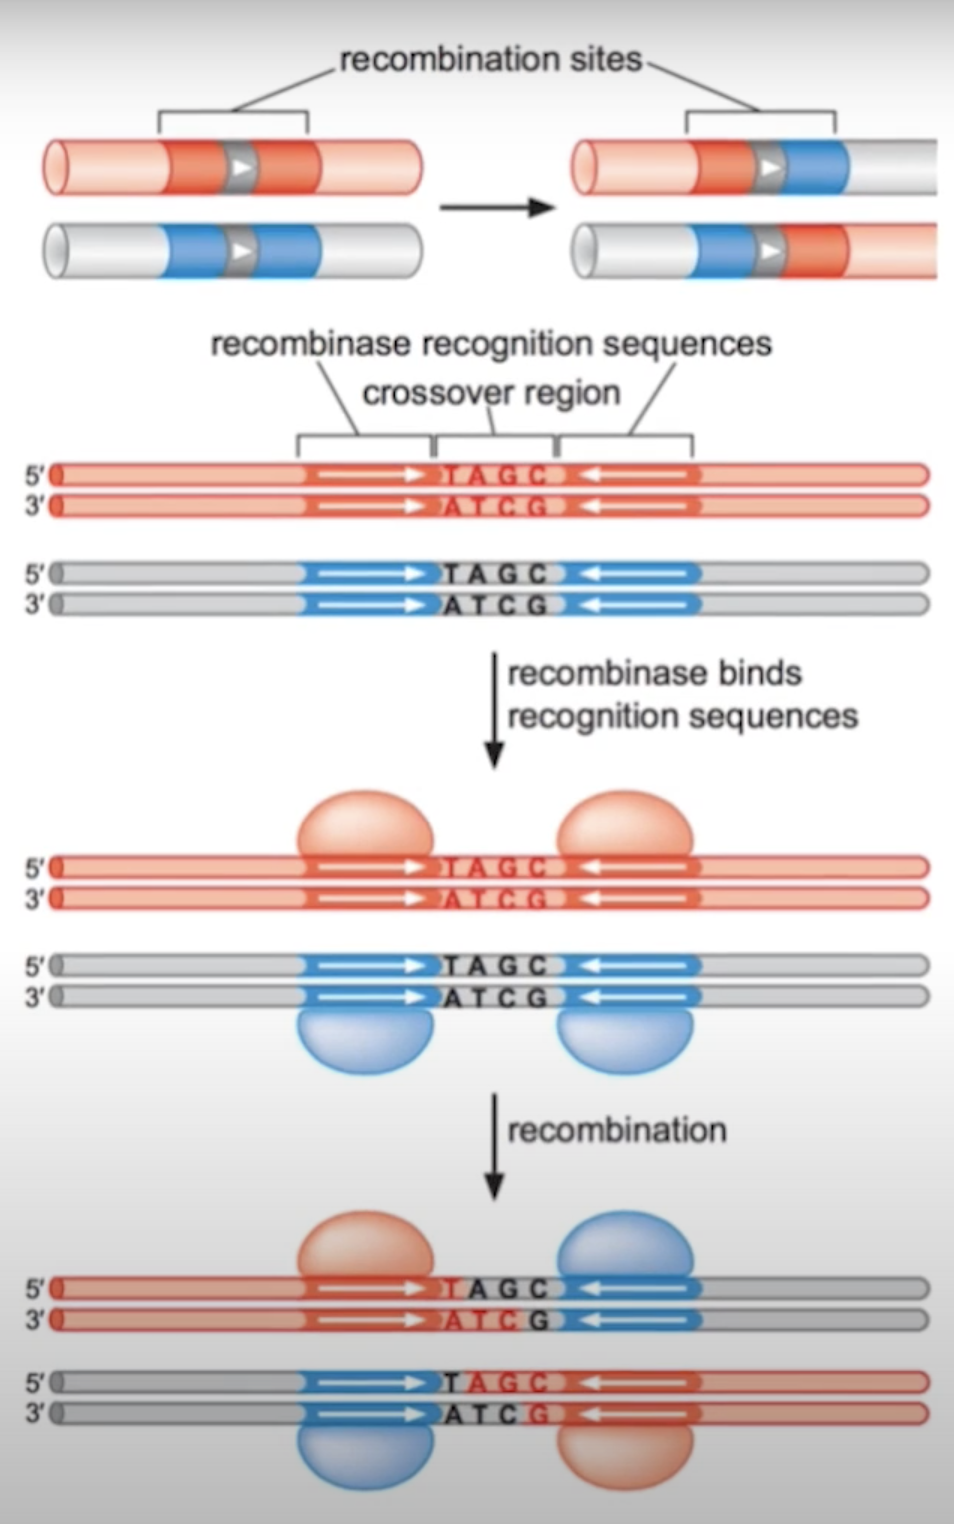
\includegraphics[scale=0.5]{8_ssrec.png}
		\caption{Сайт-специфическая рекомбинация в общем виде}
		\label{pic:8_ssrec}}
\end{figure}
\subsubsection{Транспозиция}
\textit{Я не верю в адекватность пахома, так что пусть это тут тоже будет на всякий}

Бывает нерепликативная и репликативная. Транспозоны (переезжающие куски) окружены похожими сайтами, как у сайт-специфической рекомбинации. 

\paragraph{ДНК транспозоны} Ген, необходимый для транспозиции (транспозон) окружён инвертированными концами. Дальше концов идут инвертированные концы (как палиндромы)

Инвертированные концевые повторы связываются, после них вносятся разрывы, а далее 3' концы встраиваются в ДНК, в которую будут вставляться транспозоны
 \begin{figure}[H]
	\centering{
		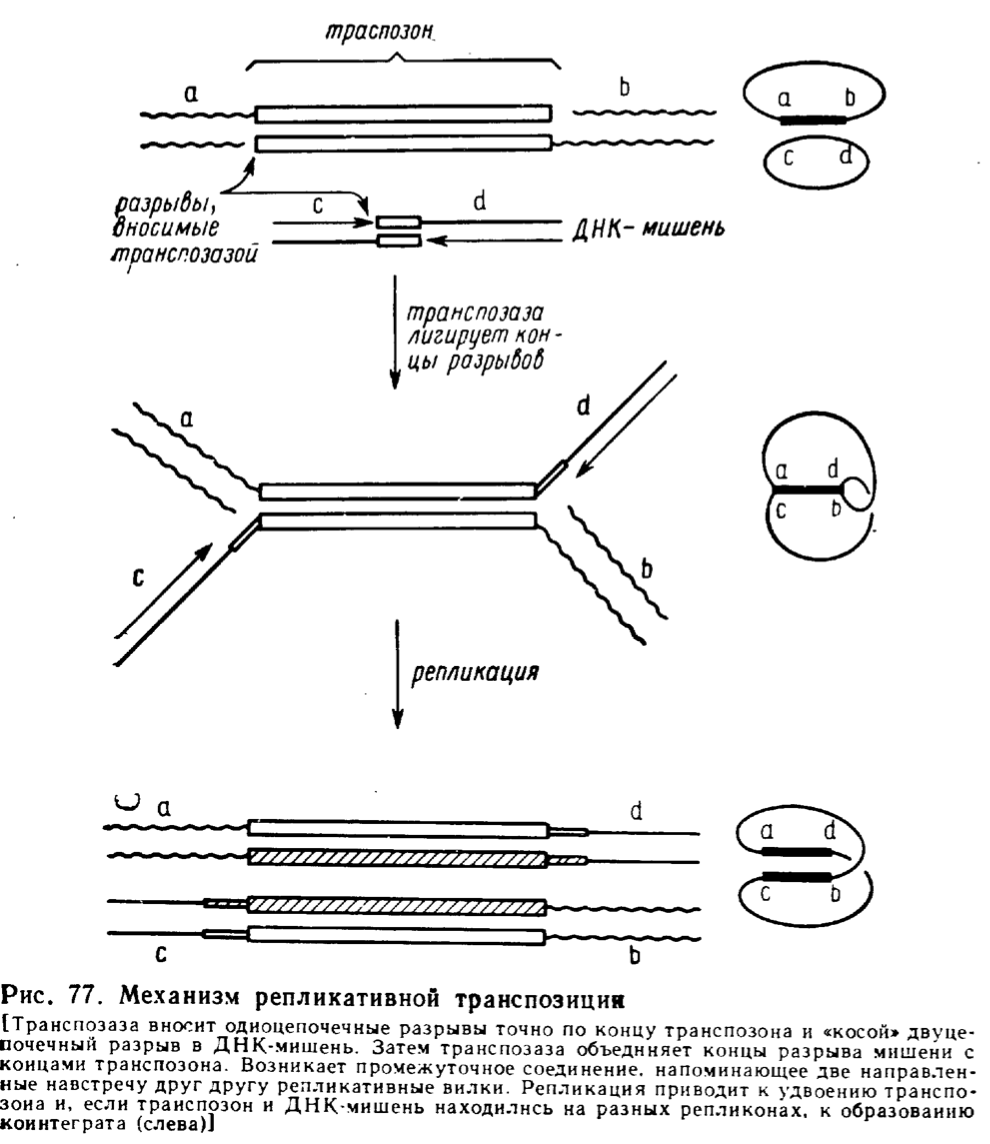
\includegraphics[scale=0.5]{8_transp.png}
		\caption{Сайт-специфическая рекомбинация в общем виде}
		\label{pic:8_transp}}
\end{figure}
\paragraph{Вирус-подобные ретропозоны} Длинные концевые повторы, потом посередине интеграза (встраивает в геном) и обратная транскриптаза. 

Сначала в ретропозоне в крайнем промоторе транскрибируется полная копия генома, потом обратной транскрипцией РНК переходит в ДНК, в котором образуются повторы, которые так же, ккак и в случае транспозонов встравиваются в днк
\section{Рекомбинация в эукариотах}
\paragraph{Мейотическая}
Перед первым делением мейоза хроматиды удерживаются вместе, но из-за кроссинговера гомологичные хромосомы тоже оказываются связаны (для правильной ориентации). Как правило рекомибанция начинается с одноцепочечного разрыва и происходит по модели Мезелсона Рэддинга (Рис \ref{pic:8_mes_red})
 \begin{figure}[H]
	\centering{
		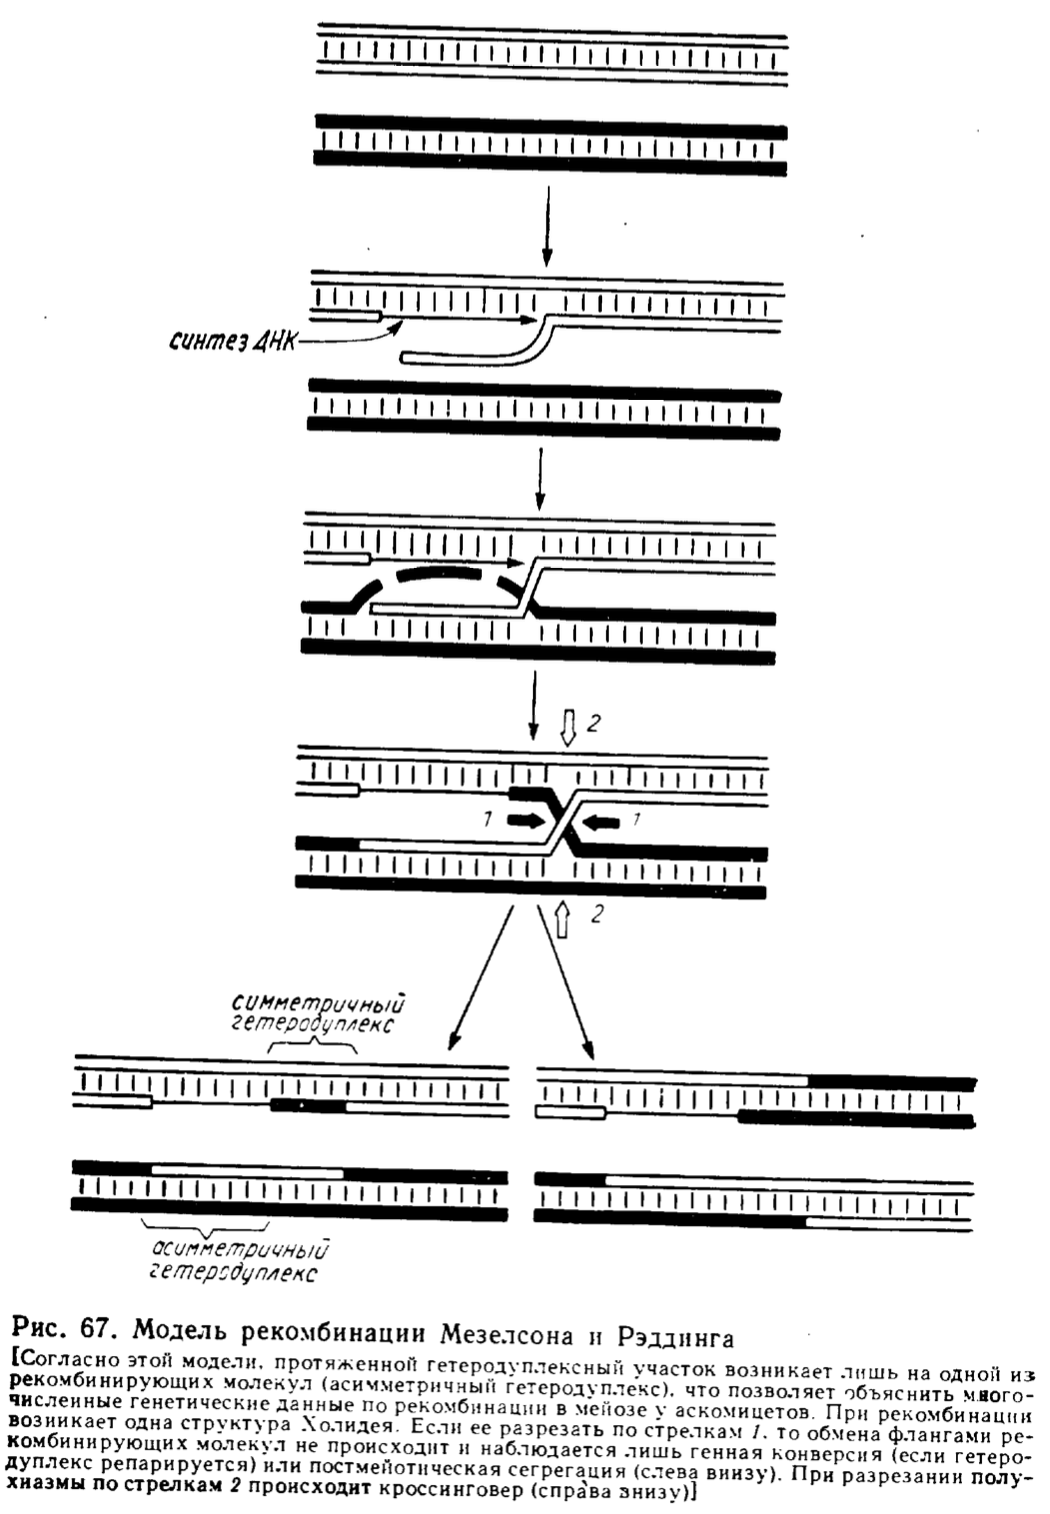
\includegraphics[scale=0.7]{8_mes_red.png}
		\caption{Мейотическая рекомбинация. Хиазм -- область связывания засчёт кроссинговера, похожая на Холидеевский крест}
		\label{pic:8_mes_red}}
\end{figure}
\paragraph{Митотическая}
Рекомбинация происходит между гомологичными генами соматических клеток многоклеточных или при вегетативном росте одноклеточных. Большинство случаев рекомбинации связаны с репарацией. Притом стимулирует рекомбинацию не только разрыв, но и двуцепочечная брешь (Рис. \ref{pic:8_eu_rec}). Характерно образование двух холидеевский крестов. Брешь при этом застраивается по образу и подобию неповреждённой молекулы. Центральную роль снова играет белок, похожий на RecA.
 \begin{figure}[H]
	\centering{
		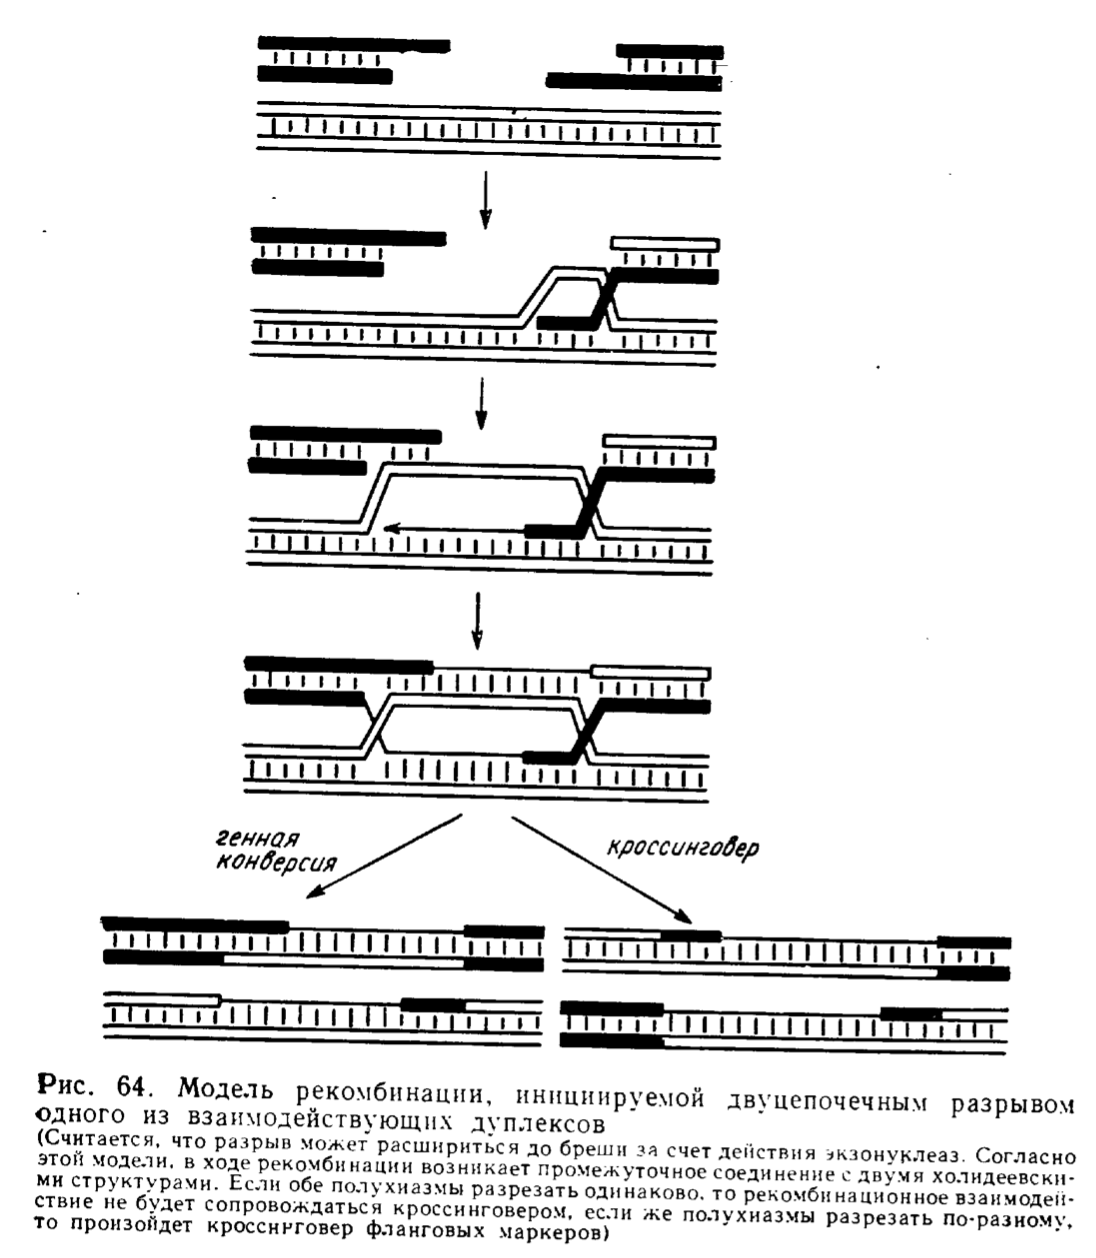
\includegraphics[scale=0.7]{8_eurec.png}
		\caption{Митотическая рекомбинация}
		\label{pic:8_eu_rec}}
\end{figure}
\paragraph{Кроссинговер} -- рекомбинационный обмена участками гомологичных хромосом во время конъюгации (их спаривание) в профазе первого деления мейоза. (Разрыв и переклеивание родительских хромосом).